% Autor: Leonhard Segger, Alexander Neuwirth
% Datum: 2017-10-30
\documentclass[
	% Papierformat
	a4paper,
	% Schriftgröße (beliebige Größen mit „fontsize=Xpt“)
	12pt,
	% Schreibt die Papiergröße korrekt ins Ausgabedokument
	pagesize,
	% Sprache für z.B. Babel
	ngerman
]{scrartcl}

% Achtung: Die Reihenfolge der Pakete kann (leider) wichtig sein!
% Insbesondere sollten (so wie hier) babel, fontenc und inputenc (in dieser
% Reihenfolge) als Erstes und hyperref und cleveref (Reihenfolge auch hier
% beachten) als Letztes geladen werden!

% Silbentrennung etc.; Sprache wird durch Option bei \documentclass festgelegt
\usepackage{babel}
% Verwendung der Zeichentabelle T1 (Sonderzeichen etc.)
\usepackage[T1]{fontenc}
% Legt die Zeichenkodierung der Eingabedatei fest, z.B. UTF-8
\usepackage[utf8]{inputenc}
% Schriftart
\usepackage{lmodern}
% Zusätzliche Sonderzeichen
\usepackage{textcomp}

% Mathepaket (intlimits: Grenzen über/unter Integralzeichen)
\usepackage[intlimits]{amsmath}
% Ermöglicht die Nutzung von \SI{Zahl}{Einheit} u.a.
\usepackage{siunitx}
% Zum flexiblen Einbinden von Grafiken (\includegraphics)
\usepackage{graphicx}
% Abbildungen im Fließtext
\usepackage{wrapfig}
% Abbildungen nebeneinander (subfigure, subtable)
\usepackage{subcaption}
% Funktionen für Anführungszeichen
\usepackage{csquotes}
% Zitieren, Bibliographie
\usepackage{biblatex}


% Zur Darstellung von Webadressen
\usepackage{url}
%chemische Formeln
\usepackage[version=4]{mhchem}
% siunitx: Deutsche Ausgabe, Messfehler getrennt mit ± ausgeben
\usepackage{floatrow}
\floatsetup[table]{capposition=top}
% Verlinkt Textstellen im PDF-Dokument
\usepackage[unicode]{hyperref}
% "Schlaue" Referenzen (nach hyperref laden!)
\usepackage{cleveref}
\sisetup{
	locale=DE,
	separate-uncertainty
}
%\bibliography{6Mi_M3_29-11-2017_References}

\begin{document}
	
	\begin{titlepage}
		\centering
		{\scshape\LARGE Versuchsbericht zu \par}
		\vspace{1cm}
		{\scshape\huge M4 - Stoßgesetze\par}
		\vspace{2.5cm}
		{\LARGE Gruppe 6Mi \par}
		\vspace{0.5cm}
		
		{\large Alexander Neuwirth (E-Mail: a\_neuw01@wwu.de) \par}
		{\large Leonhard Segger (E-Mail: l\_segg03@uni-muenster.de) \par}
		\vfill
		
		durchgeführt am 06.12.2017\par
		betreut von\par
		{\large Semir Vrana}
		
		\vfill
		
		{\large \today\par}
	\end{titlepage}
	\tableofcontents
	\newpage
	
	\section{Kurzfassung}
	%TODO Hypothese	
	%TODO Ergenisse
	%TODO 
	Um vollständig elastische Stoßprozesse durchzuführen, wurden zwei Versuche durchgeführt.
	Diese waren so konzipiert, dass sie Rückschlüsse auf den Zusammenhang zwischen den Massen und Geschwindigkeiten vor und nach einem zentralen, elastischen und geradem Stoß zulassen.
	
	\section{Methoden}
	%TODO Bilder von der Website klauen
	\subsection{Bestimmung der Massen}
	Die Massen der verwendeten drei Kugeln wurde mithilfe einer Waage gemessen.
	Dazu wurde zunächst die Waage mit aufgelegtem Ring auf Null gesetzt und dann abwechselnd die Kugeln in den Ring gelegt und die Anzeige der Waage abgelesen.
	Der Ring hatte den Zweck, die Kugeln nicht von der Waage rollen zu lassen. %Bisschen absurd ausführlich, aber idk vmtl. soll des ja so
	
	\subsection{Stoß zweier Fadenpendel} %besserer Name?
	Zwei Kugeln unterschiedlicher Masse wurden mit Seilen hintereinander aufgehängt und die Seile so justiert, dass die Schwerpunkte der Kugeln sich in der Ruhelage auf einer Höhe und in der Pendelebene befanden.
	Die Seile waren dabei jeweils an beiden Enden an einem Träger befestigt.
	Mit einem Maßband wurde die Pendellänge gemessen.
	Dann wurde für beide Pendelkugeln folgende Messung durchgeführt:
	Die Pendelkugel wurde ausgelenkt und mithilfe von verschiebbaren Markierungen auf einer Maßschiene die Auslenkung festgestellt.
	Dann wurde die Kugel losgelassen und mit einer zweiten Markierung, die nach menschlichem ermessen so platziert wurde, dass die gestoßene Kugel sie bei ihrer Schwingung gerade nicht berührte, die resultierende Auslenkung der zweiten Kugel bestimmt.
	Diese Messung wurde für fünf verschiedene Auslenkungen je fünf mal durchgeführt, um über diese Messungen mitteln zu können. %Vong deutsch her müssen Zahlen unter 13 als Wort geschrieben werden. Macht die Anleitung aber anders.
	\subsection{Stoß einer Kugel auf der Fallrinne mit einer Pendelkugel} %hmhmhm streng genommen findet der Stoß nicht auf der Fallrinne statt
	Eine kleinere Kugel wurde eine Fallrinne herunter rollen lassen und die Auslenkung einer Kugel am Fadenpendel, die von ersterer angestoßen wurde, in gleicher Art und Weise wie zuvor gemessen.
	Diese Messung wurde ebenfalls für fünf  verschiedene Starthöhen der kleinen Kugel auf der Fallrinne je fünf mal durchgeführt.
	Gemessen wurde hierbei der Abstand zum oberen Ende der Fallrinne.
	Um daraus die Starthöhe der Kugel bestimmen zu können, wurde die Fallrinne mit einer Messlatte vermessen. %Genauer muss ich hier hoffentlich nicht werden, wenn wir bei Ergebnissen ne Skizze haben.
	
	
	\section{Ergebnisse und Diskussion}
	%TODO Datenanalyse -> Überschrift?
	%TODO Unsicherheiten
	

	\subsection{Beobachtung}

	\subsubsection{Pendelstöße}
In \cref{GraphKKaufGK} und \cref{GraphGKaufKK} sind die Mittelwerte der Auslenkung nach dem Stoß von einer Kugel auf die Auslenkung der anderen Kugel aufgetragen. Der lineare Zusammenhang ist beim Betrachten der Werte bereits erkennbar und außerdem sollte dieser der Theorie zufolge auftreten (\cref{StossGleichung}). Deshalb haben wir einen Fit mit dem \enquote{Scaled Levenberg-Marquardt}-Algorithmus, welcher die Methode der kleinsten Quadrate verwendet, durchgeführt. Die Fit-Funktion sollte wie folgt aussehen: % DOppelter Afubau ??? % auf afugetragen
	\begin{equation}
		f(x)=a*x+b
	\end{equation}
	
	\begin{equation}
		\label{StossGleichung}
		a_2' = a_1 \frac{2m_1}{m_1+m_2} = a_1 m(a_2')
	\end{equation}
	Wenn man die Steigungen der Auslenkungen $a_2'$ und $a_1'$ addiert erhält man:
	\begin{equation}
		m(a_2') + m(a_1') = \frac{2m_1}{m_1+m_2} + \frac{2m_2}{m_2+m_1} = 2
	\end{equation}
	Die Summe der Steigungen (\cref{TabelleFits}) der linearen Fit-Funktionen beträgt \SI{1,87}{}
	 
	\begin{table}[tb]
	\centering
	\begin{tabular}{ l | c | c | }
		& Kleine stößt Große $a_1$ & Große stößt Kleine $a_2$ \\ \hline 
		m &  $\SI{0,5038 \pm 0,0147}{}$ &$\SI{1,3744 \pm 0,0203}{}$  \\ \hline
	\end{tabular}
	\caption{Steigungen die sich beim Fitten ergeben.}
	\label{TabelleFits}
	\end{table}
	Aus den Steigungen lässt sich das Verhältnis der Massen bestimmen.
	\begin{align}
		k = \frac{m(a_2')}{m(a_1')} = \frac{2m_1}{m_1+m_2} \frac{m_1+m_2}{2m_2} = \frac{m_1}{m_2} \\
		u(k) =  k \sqrt{\left(\frac{u(m(a_1'))}{m(a_1')}\right)^2 + \left(\frac{u(m(a_2'))}{m(a_2')}\right)^2 }
	\end{align}
	Es ergibt sich eine Massenverhältnis von $k_s$ =  \SI{2,7281 \pm 0,089}{}. In \cref{MessungGewichte} sind die gewogenen Massen der Kugeln aufgeführt. Das Massenverhältnis ist $k_m$ = $\SI{3,0182 \pm 6,66 }{}$. 
	%TODO Unsichcerheite
	\begin{table}[tb]
	\centering
	\begin{tabular}{ l | c | c | }
		& Große Kugel & kleine Kugel \\ \hline 
		Masse &  $\SI{192,26 \pm 6,66}{g}$ &$\SI{63,70 \pm 6,66}{g}$  \\ \hline %TODO Unsichcerheite
	\end{tabular}
	\caption{Masse die sich beim Wiegen der Kugel ergeben.}
	\label{MessungGewichte}
	\end{table}
	


	\begin{figure}[htb]
	  \centering
	    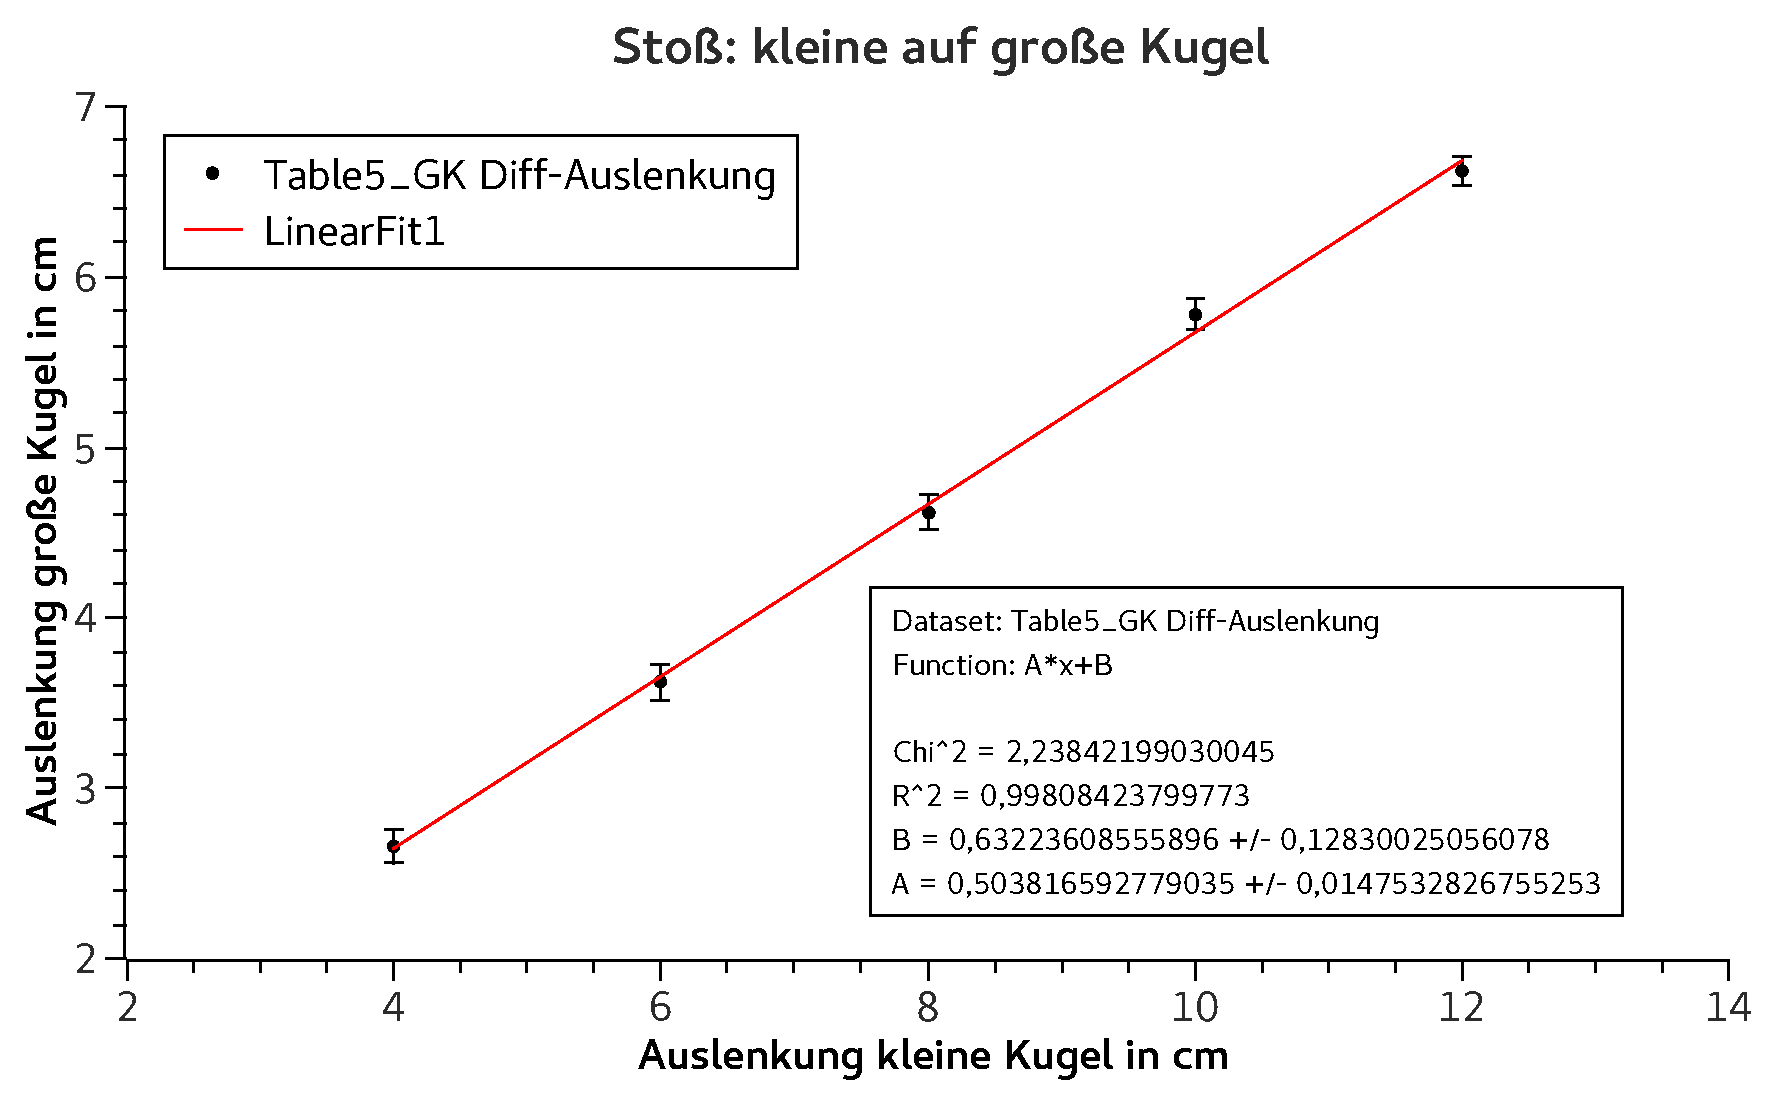
\includegraphics[width=0.8\textwidth]{StossKKaufGK} % Keine Angabe der Dateiendung nötig, TeX durchsucht den Ordner, in dem dieser Quelltext liegt
	  \caption{Kleine Kugel stößt die große Kugel.}
		\label{GraphKKaufGK}
	\end{figure}
		
	\begin{figure}[htb]
	  \centering
	    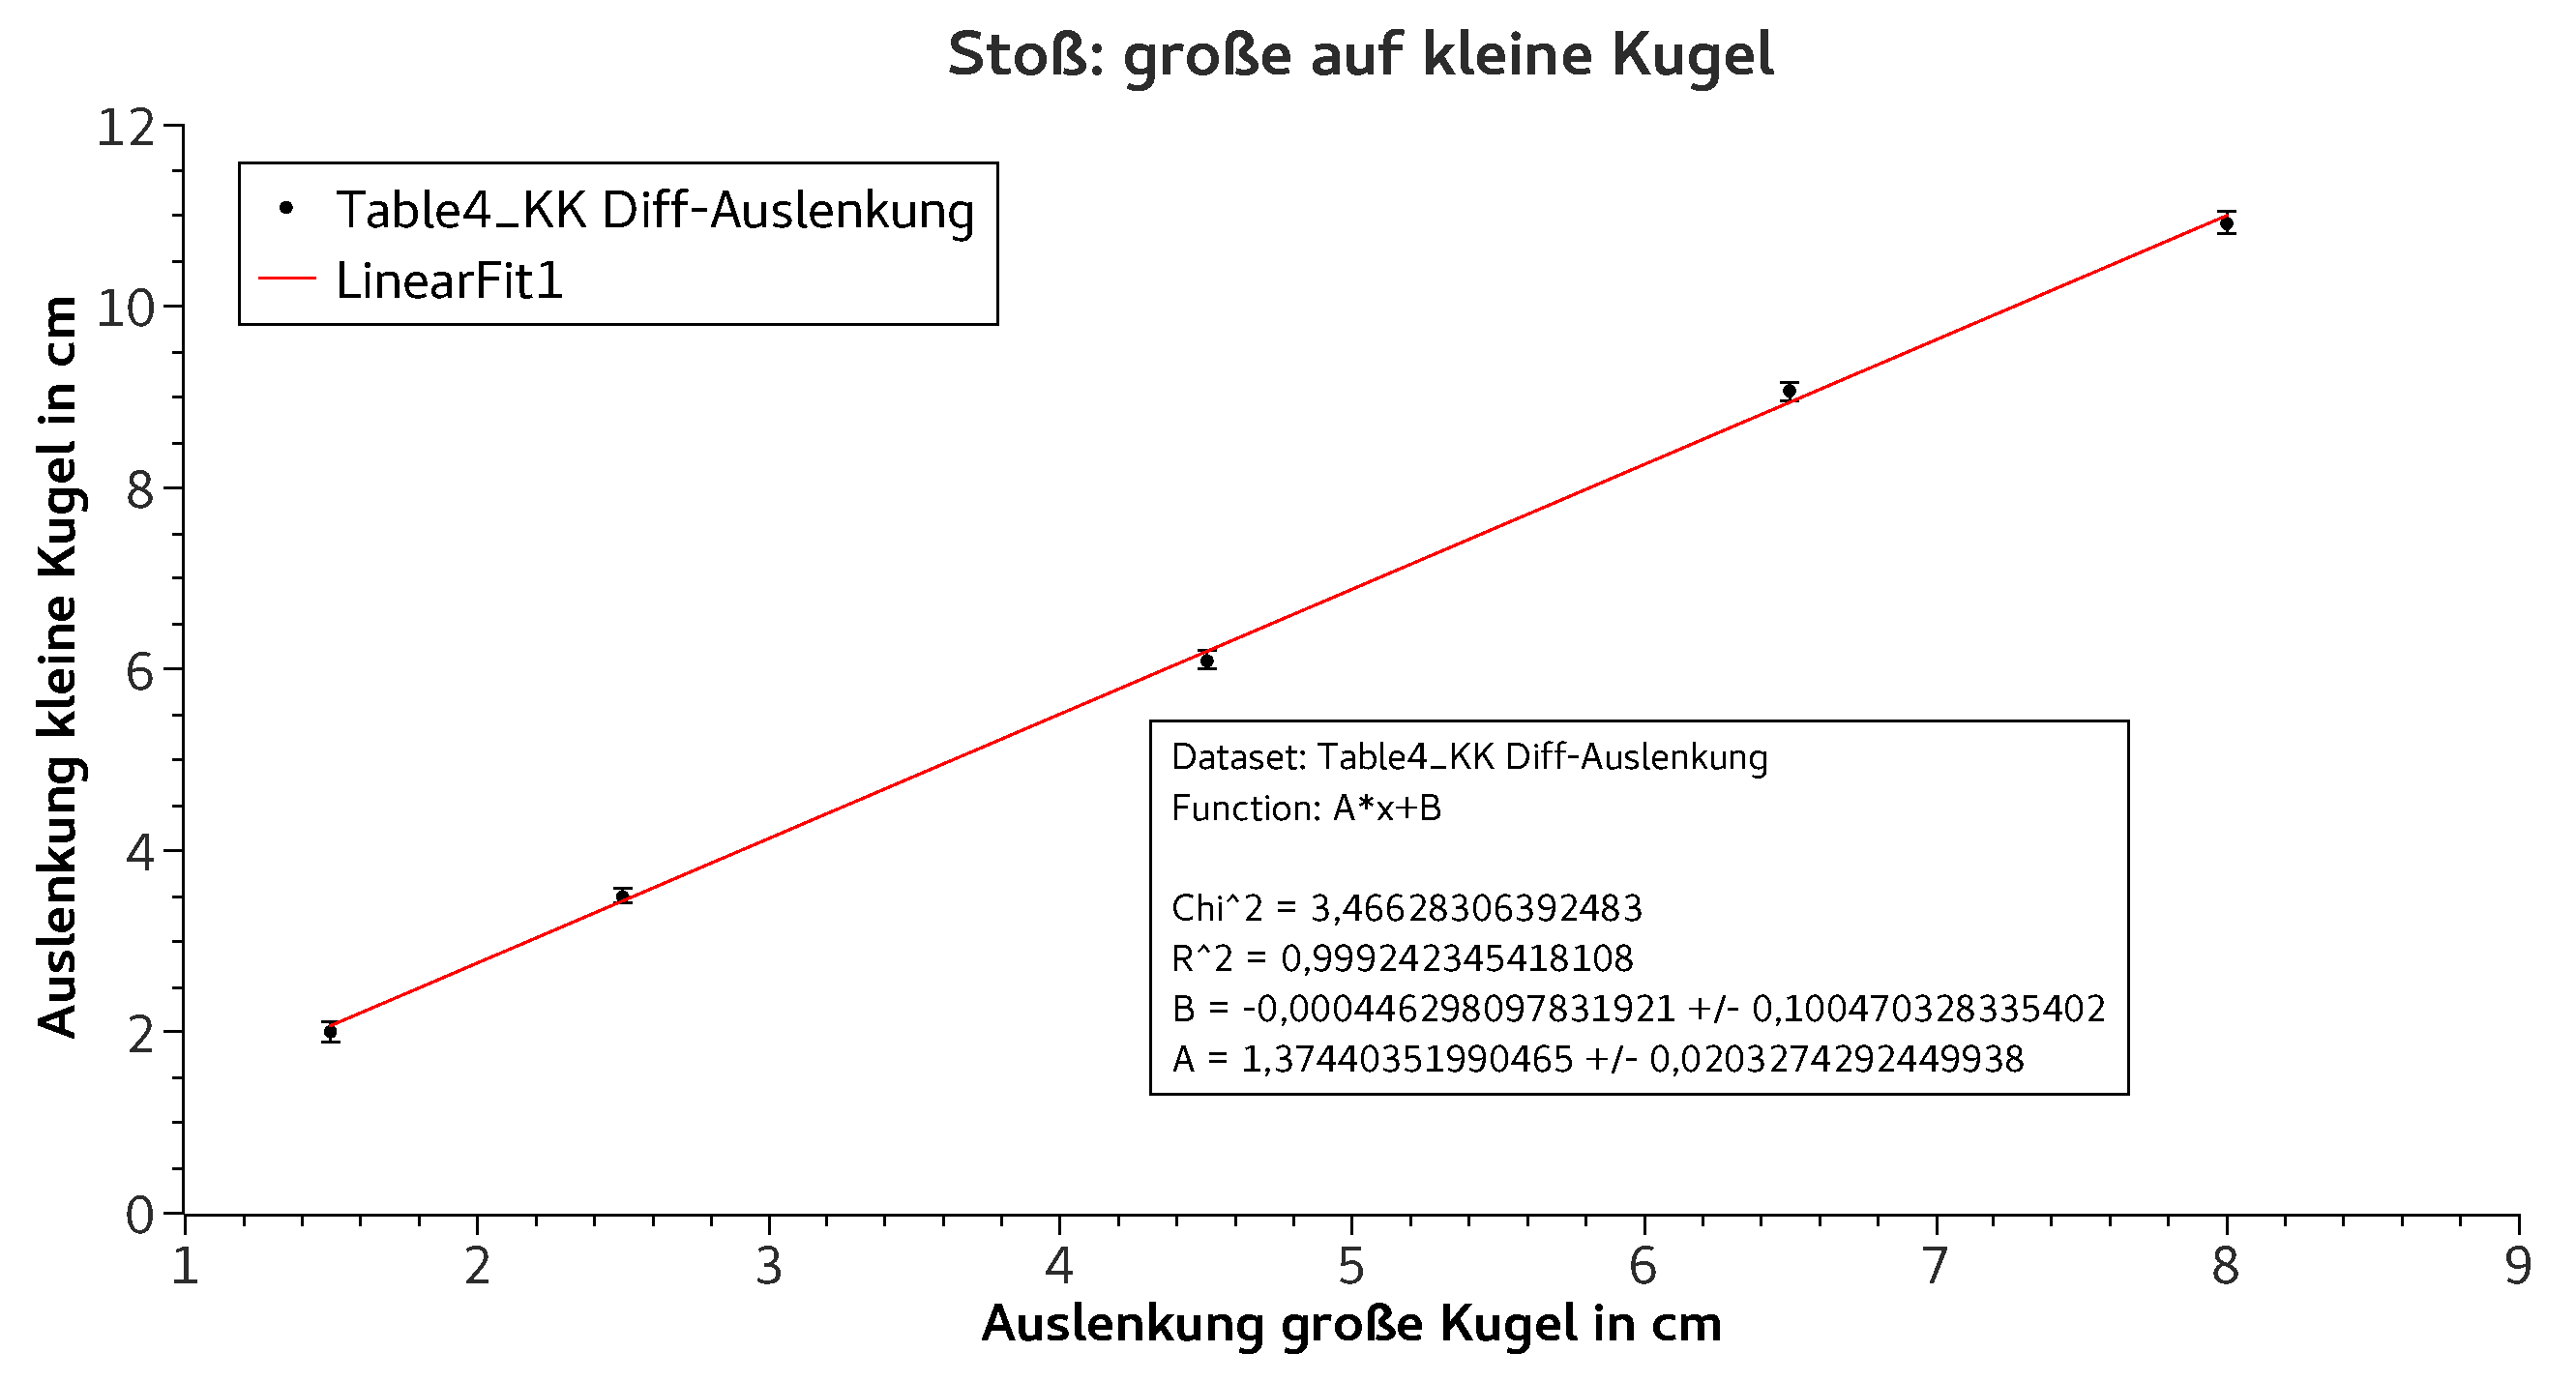
\includegraphics[width=0.8\textwidth]{StossGKaufKK} % Keine Angabe der Dateiendung nötig, TeX durchsucht den Ordner, in dem dieser Quelltext liegt
	  \caption{Große Kugel stößt die kleine Kugel.}
		\label{GraphGKaufKK}
	\end{figure}


	\subsubsection{Fallrinne}
	Aus den Abbmessungen $H$, $L$ und $h_0$ der Fallrinne (vgl. Abb. 2 der Einführung) lässt sich die Fallhöhe wie folgt bestimmen. Aus der Skizze ist ersichtlich, dass 
	\begin{equation}
		\sin(\alpha) s = h_0-h 
		\label{Sin1}
	\end{equation}
	und
	\begin{equation}
		\sin(\alpha) = \frac{H}{S} = \frac{H}{\sqrt{H^2+L^2}} = \frac{1}{\sqrt{1+L^2/H^2}}
		\label{Sin2}
	\end{equation}
	gilt. Fügt man \cref{Sin1} und \cref{Sin2} zusammen erhält man:
	\begin{equation}
		h = h_0 - \frac{s}{\sqrt{1+ L^2/H^2}}
	\end{equation}
	\subsection{Diskussion}
	%TODO 
	%TODO Diskussion von Steigungs summe 1,87. Auffällig das Beide Steiguingen ca. gleich niederer als MAsse calculation

	\section{Schlussfolgerung}
	%TODO Rückgriff auf Hypothese
	
	%TODO Quellen zitieren, Websiten mit Zugriffsdatum
	%TODO Verweise auf das Laborbuch (sind erlaubt)
	%TODO Tabelle + Bilder mit Beschriftung
	%\printbibliography
\end{document}
